\documentclass[aspectratio=169]{beamer}
\usetheme{Madrid}
\usecolortheme{beaver}
\usepackage[utf8]{inputenc}
\usepackage[T1]{fontenc}
\usepackage{tikz}
\usepackage{amssymb}
\usepackage{graphicx}
\setbeamertemplate{navigation symbols}{}
\setbeamercolor{title}{fg=white,bg=cyan!60!black}
\setbeamercolor{frametitle}{fg=white,bg=cyan!50!black}
\setbeamercolor{block title}{bg=cyan!15,fg=black}
\setbeamercolor{block body}{bg=cyan!5,fg=black}

\title{Story Studio 4 — Remember Things}
\subtitle{Lesson 1: Remember the Choice}
\author{ByteForge --- Grade 7 --- Game Maker}
\date{}

\begin{document}

\begin{frame}
    \titlepage
\end{frame}

\begin{frame}{A variable is a box with a name}
    \Large
    A named box holding a value your code can reuse, combine, or change later — the same code works no matter what's stored inside.

    \begin{center}
    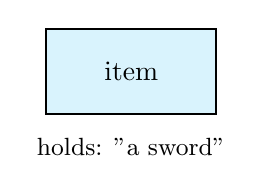
\begin{tikzpicture}[scale=0.9]

        \draw[thick, fill=cyan!15] (0,0) rectangle (2.4,-1.2);
        \node at (1.2,-0.6) {item};
        \node[below] at (1.2,-1.4) {\small holds: "a sword"};
    \end{tikzpicture}
    \end{center}
\end{frame}

\begin{frame}{Your Turn}
    \Large
    Open the student map, find \textbf{Story Studio 4 — Remember Things}, and complete
    the \textbf{Remember the Choice} challenge --- everything you just saw, they now do themselves.
\end{frame}

\end{document}
